%% abtex2-modelo-trabalho-academico.tex, v-1.7.1 laurocesar
%% Copyright 2012-2013 by abnTeX2 group at http://abntex2.googlecode.com/ 
%%
%% This work may be distributed and/or modified under the
%% conditions of the LaTeX Project Public License, either version 1.3
%% of this license or (at your option) any later version.
%% The latest version of this license is in
%%   http://www.latex-project.org/lppl.txt
%% and version 1.3 or later is part of all distributions of LaTeX
%% version 2005/12/01 or later.
%%
%% This work has the LPPL maintenance status `maintained'.
%% 
%% The Current Maintainer of this work is the abnTeX2 team, led
%% by Lauro César Araujo. Further information are available on 
%% http://abntex2.googlecode.com/
%%
%% This work consists of the files abntex2-modelo-trabalho-academico.tex,
%% abntex2-modelo-include-comandos and abntex2-modelo-references.bib
%%

% ------------------------------------------------------------------------
% ------------------------------------------------------------------------
% abnTeX2: Modelo de Trabalho Academico (tese de doutorado, dissertacao de
% mestrado e trabalhos monograficos em geral) em conformidade com 
% ABNT NBR 14724:2011: Informacao e documentacao - Trabalhos academicos -
% Apresentacao
% ------------------------------------------------------------------------
% ------------------------------------------------------------------------

\documentclass[
  % -- opções da classe memoir --
  12pt,       % tamanho da fonte
  openright,      % capítulos começam em pág ímpar (insere página vazia caso preciso)
  twoside,      % para impressão em verso e anverso. Oposto a oneside
  a4paper,      % tamanho do papel. 
  % -- opções da classe abntex2 --
  %chapter=TITLE,   % títulos de capítulos convertidos em letras maiúsculas
  %section=TITLE,   % títulos de seções convertidos em letras maiúsculas
  %subsection=TITLE,  % títulos de subseções convertidos em letras maiúsculas
  %subsubsection=TITLE,% títulos de subsubseções convertidos em letras maiúsculas
  % -- opções do pacote babel --
  english,      % idioma adicional para hifenização
  brazil,       % o último idioma é o principal do documento
  ]{abntex2}


% ---
% PACOTES
% ---

% ---
% Pacotes fundamentais 
% ---
\usepackage{cmap}       % Mapear caracteres especiais no PDF
\usepackage{lmodern}      % Usa a fonte Latin Modern
\usepackage[T1]{fontenc}    % Selecao de codigos de fonte.
\usepackage[utf8]{inputenc}   % Codificacao do documento (conversão automática dos acentos)
\usepackage{lastpage}     % Usado pela Ficha catalográfica
\usepackage{indentfirst}    % Indenta o primeiro parágrafo de cada seção.
\usepackage{color}        % Controle das cores
\usepackage{graphicx}     % Inclusão de gráficos
\usepackage{xspace}
\usepackage{fourier} 
\usepackage{array}
\usepackage{makecell}
\usepackage{graphics}
% ---

% Pacotes extras
\usepackage[table,xcdraw]{xcolor}   % Inclusão de cores em tabelas
\usepackage{todonotes}
\usepackage{multirow}
\usepackage{pdfpages}
% % Abreviações
% \newcommand{\Fw}{\textit{Framework}\xspace}
% \newcommand{\fw}{\textit{framework}\xspace}
% \newcommand{\Fws}{\textit{Frameworks}\xspace}
% \newcommand{\fws}{\textit{frameworks}\xspace}

% \newcommand{\pskel}{{\small \textsf{PSkel}}\xspace}
% \newcommand{MPPA-256}{{\small \textsf{MPPA-256}}\xspace}

% Acronyms
\usepackage[acronym,nowarn]{glossaries}

\glsdisablehyper

%%%%%%%%%%%%%%%%%%%%%%%%%%%%%%%%%%%%%%%%%%%%%%%%%%%%%%%%%%%%%%%%%%%%
%%% Acronyms list                                                %%%
%%%%%%%%%%%%%%%%%%%%%%%%%%%%%%%%%%%%%%%%%%%%%%%%%%%%%%%%%%%%%%%%%%%%
%%% Importante:                                      
%%% - A lista PRECISA SER MANTIDA ORDENADA
%%%%%%%%%%%%%%%%%%%%%%%%%%%%%%%%%%%%%%%%%%%%%%%%%%%%%%%%%%%%%%%%%%%%

%A
\xnewacronym[amp]{AMP}{Asymmetric Multi-Processing}
\xnewacronym[anova]{ANOVA}{Analysis of Variance}
\xnewacronym[api]{API}{Application Programming Interface}

%B

%C
\xnewacronym[cnoc]{C-NoC}{Control Network-on-Chip}
\xnewacronym[cmp]{CMP}{Chip Multiprocessor}
\xnewacronym[cow]{COW}{Copy-On-Write}
\xnewacronym[cpu]{CPU}{Central Processing Unit}

%D
\xnewacronym[dnoc]{D-NoC}{Data Network-on-Chip}
\xnewacronym[dma][longplural={Direct Memory Accesses}]{DMA}{Direct Memory Access}
\xnewacronym[dram][longplural={Dynamic Random Access Memories}]{DRAM}{Dynamic Random Access Memory}
\xnewacronym[dtlb]{DTLB}{Data Translation Lookaside Buffer}

%E

%F
\xnewacronym[flops]{FLOPS}{\textit{Floating-point Operations per Second}}
\xnewacronym[fos]{FOS}{Factored Operating System}
\xnewacronym[fpga]{FPGA}{Field Programmable Gate Array}

%G
\xnewacronym[gpu]{GPU}{Graphics Processing Unit}

%H
\xnewacronym[hal]{HAL}{Hardware Abstraction Layer}
\xnewacronym[hpc]{HPC}{High-Performance Computing}

%I
\xnewacronym[iid]{i.i.d}{Independent and Identically Distributed}
\xnewacronym[ipc]{IPC}{Inter-Process Communication}
\xnewacronym[isa]{ISA}{Distributed Hash Table}
\xnewacronym[itlb]{ITLB}{Instruction Translation Lookaside Buffer}
\xnewacronym[ieee]{IEEE}{Institute of Electrical and Electronics Engineers}

%J
\xnewacronym[jtlb]{JTLB}{Join Translation Lookaside Buffer}

%K

%L
\xnewacronym[lfour]{L4}{L4 Microkernel}
\xnewacronym[ltlb]{LTLB}{Locked Translation Lookaside Buffer}

%M
\xnewacronym[mimd]{MIMD}{Multiple Instruction Multiple Data}
\xnewacronym[misd]{MISD}{Multiple Instruction Single Data}
\xnewacronym[mmio]{MMIO}{Memory-Mapped I/O}
\xnewacronym[mmu]{MMU}{Memory Management Unit}
\xnewacronym[moosca]{MOOSCA}{Manycore Operating System for Safety-Critical Application}
\xnewacronym[mos]{mOS}{multi Operating System}
\xnewacronym[mpsoc]{MPSoC}{Multiprocessor System-on-Chip}
\xnewacronym[mpu]{MPU}{Memory Protection Unit}

%N
\xnewacronym[noc]{NoC}{Network-on-Chip}
\xnewacronym[norma]{NoRMA}{No Remote Memory Access}
\xnewacronym[nos]{nOS}{Nano-Sized Operating System}
\xnewacronym[numa]{NUMA}{Non-Uniform Memory Access}

%O
\xnewacronym[os]{OS}{Operating System}

%P
\xnewacronym[pe]{PE}{Processing Element}
\xnewacronym[pgas]{PGAS}{Partitioned Global Address Space}
\xnewacronym[pmca]{PMCA}{Programmable Manycore Accelerator}
\xnewacronym[pmio]{PMIO}{Port-Mapped I/O}
\xnewacronym[posix]{POSIX}{Portable Operating System Interface}

%Q
\xnewacronym[qos]{QoS}{Quality of Service}

%R
\xnewacronym[rab]{RAB}{Remapping Address Block}
\xnewacronym[ram][longplural={Random Access Memories}]{RAM}{Random Access Memory}
\xnewacronym[risc]{RISC}{Reduced Instruction Set Computer}
\xnewacronym[rm]{RM}{Resource Manager}
\xnewacronym[rma][longplural={Remote Memory Accesses}]{RMA}{Remote Memory Access}
\xnewacronym[rmem][longplural={Remote Memories}]{RMem}{Remote Memory}

%S
\xnewacronym[simd]{SIMD}{Single Instruction Multiple Data}
\xnewacronym[sisd]{SISD}{Single Instruction Single Data}
\xnewacronym[shm]{SHM}{POSIX Shared Memory}
\xnewacronym[smp]{SMP}{Symmetric Multi-Processing}
\xnewacronym[soc]{SoC}{System-on-a-Chip}
\xnewacronym[spm][longplural={Software-managed Scratchpad Memories}]{SPM}{Software-managed Scratchpad Memory}
\xnewacronym[sram][longplural={Static Random Access Memories}]{SRAM}{Static Random Access Memory}
	
%T
\xnewacronym[tlb]{TLB}{Translation Lookaside Buffer}

%U
\xnewacronym[uma][longplural={Uniform Memory Accesses}]{UMA}{Uniform Memory Access}

%V
\xnewacronym[vliw]{VLIW}{Very Long Instruction Word}

%W
\xnewacronym[watts]{W}{\textit{Watts}}

%%% Local Variables:
%%% mode: latex
%%% TeX-master: "main"
%%% End:

% \makeglossaries
% ---
% Pacotes adicionais, usados apenas no âmbito do Modelo Canônico do abnteX2
% ---
\usepackage{lipsum}       % para geração de dummy text
% ---

% ---
% Pacotes de citações
% ---
%\usepackage[brazilian,hyperpageref]{backref}  % Paginas com as citações na bibl
\usepackage[alf]{abntex2cite}                  % Citações padrão ABNT
% --- 
% CONFIGURAÇÕES DE PACOTES
% --- 

% ---
% Configurações do pacote backref
% Usado sem a opção hyperpageref de backref
%\renewcommand{\backrefpagesname}{Citado na(s) página(s):~}
% Texto padrão antes do número das páginas
%\renewcommand{\backref}{}
% Define os textos da citação
%\renewcommand*{\backrefalt}[4]{
% \ifcase #1 %
%   Nenhuma citação no texto.%
% \or
%   Citado na página #2.%
% \else
%   Citado #1 vezes nas páginas #2.%
% \fi}%
% ---

% ---
% Informações de dados para CAPA e FOLHA DE ROSTO
% ---
\titulo{Desenvolvimento de um \textit{Exokernel} para o Processador \textit{Manycore} MPPA-256}
% \titulo{Desenvolvimento de um Lightweight Exokernel para o Processador Manycore MPPA-256}
\autor{João Vicente Souto}
\local{Florianópolis}
\data{2018}
\orientador{Márcio Bastos Castro}
\coorientador{Pedro Henrique Penna}
\instituicao{%
  Universidade Federal de Santa Catarina
  \par
  Departamento de Informática e Estatística
  \par
  Ciência da Computação}
\tipotrabalho{Trabalho de Conclusão de Curso de Graduação}
% O preambulo deve conter o tipo do trabalho, o objetivo, 
% o nome da instituição e a área de concentração 
\preambulo{Proposta de monografia submetida ao Programa
de Graduação em Ciência da Computação
para a obtenção do Grau de Bacharel.}
% ---


% ---
% Configurações de aparência do PDF final

% alterando o aspecto da cor azul
\definecolor{blue}{RGB}{41,5,195}

% informações do PDF
\makeatletter
\hypersetup{
      %pagebackref=true,
    pdftitle={\@title}, 
    pdfauthor={\@author},
      pdfsubject={\imprimirpreambulo},
      pdfcreator={LaTeX with abnTeX2},
    pdfkeywords={abnt}{latex}{abntex}{abntex2}{trabalho acadêmico}, 
    hidelinks,
    colorlinks=false,         % false: boxed links; true: colored links
      linkcolor=blue,           % color of internal links
      citecolor=blue,           % color of links to bibliography
      filecolor=magenta,        % color of file links
    urlcolor=blue,
    bookmarksdepth=4
}
\makeatother
% --- 

% --- 
% Espaçamentos entre linhas e parágrafos 
% --- 

% O tamanho do parágrafo é dado por:
\setlength{\parindent}{1.3cm}

% Controle do espaçamento entre um parágrafo e outro:
\setlength{\parskip}{0.2cm}  % tente também \onelineskip

% ---
% compila o indice
% ---
\makeindex
% ---

% ----
% Início do documento
% ----
\begin{document}

% Retira espaço extra obsoleto entre as frases.
\frenchspacing 

% ----------------------------------------------------------
% ELEMENTOS PRÉ-TEXTUAIS
% ----------------------------------------------------------
% \pretextual

% ---
% Capa
% ---
\imprimircapa
% ---

% ---
% Folha de rosto
% (o * indica que haverá a ficha bibliográfica)
% ---
\imprimirfolhaderosto*
% ---

% ---
% Inserir a ficha bibliografica
% ---

% Isto é um exemplo de Ficha Catalográfica, ou ``Dados internacionais de
% catalogação-na-publicação''. Você pode utilizar este modelo como referência. 
% Porém, provavelmente a biblioteca da sua universidade lhe fornecerá um PDF
% com a ficha catalográfica definitiva após a defesa do trabalho. Quando estiver
% com o documento, salve-o como PDF no diretório do seu projeto e substitua todo
% o conteúdo de implementação deste arquivo pelo comando abaixo:
%
% % \begin{fichacatalografica}
% %     \includepdf{fig_ficha_catalografica.pdf}
% % \end{fichacatalografica}
% \begin{fichacatalografica}
%   \vspace*{\fill}         % Posição vertical
%   \hrule              % Linha horizontal
%   \begin{center}          % Minipage Centralizado
%   \begin{minipage}[c]{12.5cm}   % Largura
  
%   Podestá Junior, Emmanuel
  
%   \hspace{0.5cm} \imprimirtitulo \ / \imprimirautor;  \imprimirorientadorRotulo~\imprimirorientador; \imprimirlocal, \imprimirdata-
  
%   \hspace{0.5cm} \pageref{LastPage} p. : il. (algumas color.) ; 30 cm.\\
  
%   %\hspace{0.5cm} \imprimirorientadorRotulo~\imprimirorientador, Coorientador: Daniel Priori \\
  
%   \hspace{0.5cm}
%   \imprimirtipotrabalho \ --\ Universidade Federal de Santa Catarina, Departamento de Informática e Estatística, Ciência da Computação,
%   \imprimirdata.\\
  
% %   \hspace{0.5cm} Inclui referências \\
  
% %   \hspace{0.5cm}
% %     1. Ciência da Computação.
% %     2. Inteligência Artificial.
% %     3. Deep Learning.
% %     I. Mauro Roisenberg.
% %     II. Daniel Priori.
% %     III. Universidade Federal de Santa Catarina.
% %     IV. Título \\       
  
%   %\hspace{8.75cm} CDU 02:141:005.7\\
  
%   \end{minipage}
%   \end{center}
%   \hrule
% \end{fichacatalografica}
% ---

% ---
% Inserir folha de aprovação
% ---

% Isto é um exemplo de Folha de aprovação, elemento obrigatório da NBR
% 14724/2011 (seção 4.2.1.3). Você pode utilizar este modelo até a aprovação
% do trabalho. Após isso, substitua todo o conteúdo deste arquivo por uma
% imagem da página assinada pela banca com o comando abaixo:
%
% \includepdf{folhadeaprovacao_final.pdf}
%
\begin{folhadeaprovacao}

%  \begin{center}
%    {\ABNTEXchapterfont\bfseries\Large FOLHA DE APROVAÇÃO DE PROPOSTA DO TCC}
%    %\hspace{.45\textwidth}
%    %\begin{minipage}{.5\textwidth}
%        %\imprimirpreambulo
%    %\end{minipage}
%    %\vspace*{\fill}
%   \end{center}
%   \renewcommand\theadalign{cb}
%   \renewcommand\theadfont{\bfseries}
% \renewcommand\theadgape{\Gape[4pt]}
% \renewcommand\cellgape{\Gape[4pt]}
%   %\def\arraystretch{2}%  1 is the default, change whatever you need
% \begin{flushleft}
%    \resizebox{\columnwidth}{!}{%
% \begin{tabular}{|l|l|}
% \hline
%     \textbf{Acadêmico(s)} &  João Vicente Souto \hspace{74mm} \\ \hline
%            \textbf{Título do Trabalho}  & \makecell[l]{PSkel-MPPA: Uma Adaptação do Framework PSkel para \\ o Processador Manycore %MPPA-256}\\ \hline
%            \textbf{Curso} & Ciências da Computação/INE/UFSC \\ \hline
%            \textbf{Área de Concentração} & \textbf{DETERMINAR ÁREAS DE CONCENTRAÇÃO} \\ \hline
%    \end{tabular}
%    }
%    \end{flushleft}
%    \begin {flushleft}
%    \textbf{Instruções para preenchimento pelo \emph{ORIENTADOR DO TRABALHO}:}
%    \begin{itemize}
%    \item Para cada critério avaliado, assinale um X na coluna SIM apenas se considerado aprovado. Caso contrário, indique as alterações %necessárias na coluna de Observação.
%    \end{itemize}
%    \end{flushleft}
%    \newcolumntype{C}{>{\centering\arraybackslash}p{25em}}
%    \newcolumntype{A}{>{\centering\arraybackslash}p{4em}}
%    \newcolumntype{O}{>{\centering\arraybackslash}p{11em}}
%    \begin{flushleft}
%    \resizebox{\columnwidth}{!}{%
%    \begin{tabular}{|C|A|A|A|A|O|}
%    \hline
%     \multirow{2}{*}{\textbf{Critérios}} & \multicolumn{4}{c|}{\textbf{Aprovado}} & \multirow{2}{*}{\textbf{Observação}} \\[1ex]
% \cline{2-5}
%        & \textbf{Sim} & \textbf{Parcial} & \textbf{Não} & \textbf{Não se aplica} & \\
%        \hline
%        \makecell[l]{O trabalho é adequado para um TCC em CCO \\ (relevância / abrangência)?}& & & & & \\
%        \hline
%        \makecell[l]{O título é adequado?}& & & & & \\
%        \hline
%        \makecell[l]{O Tema de pesquisa está claramente descrito?}& & & & & \\
%        \hline
%        \makecell[l]{O problema/hipóteses de pesquisa do trabalho está \\ claramente identificado?}& & & & & \\
%        \hline
%        \makecell[l]{A relevância da pesquisa é justificada?}& & & & & \\
%        \hline
%        \makecell[l]{Os objetivos descrevem completa e claramente o \\ que se pretende alcançar neste trabalho?}& & & & & \\
%        \hline
%        \makecell[l]{É definido o método a ser adotado no trabalho? \\ O método condiz com os objetivos e é adequado \\ para um TCC?}& & %& & & \\
%        \hline
%        \makecell[l]{Foi definido um cronograma coerente com o método\\ definido (indicando todas as atividades) e com as \\ datas das %entregas (p.ex. Projeto I, II, Defesa)?}& & & & & \\
%        \hline
%        \makecell[l]{Foram identificados custos relativos à execução deste \\ trabalho (se houver)? Haverá financiamento para \\ estes %custos?}& & & & & \\
%        \hline
%        \makecell[l]{Foram identificados todos os envolvidos neste \\ trabalho?}& & & & & \\
%        \hline
%        \makecell[l]{As formas de comunicação foram definidas?}& & & & & \\[1ex]
%        \hline
%        \makecell[l]{Riscos potenciais que podem causar desvios do plano \\ foram identificados?}& & & & & \\
%        \hline
%        \makecell[l]{Caso o TCC envolva a produção de um software ou \\ outro tipo de produto e seja desenvolvido também \\ como uma %atividade realizada numa empresa ou \\ laboratório, consta na proposta uma declaração\\ (Anexo 3) de ciência e concordância com a %entrega\\ do código fonte e/ou documentação produzidos?}& & & & & \\
%        \hline
%    \end{tabular}
%    }
%    \newcolumntype{B}{>{\centering\arraybackslash}p{41.72em}}
%    \newcolumntype{E}{>{\centering\arraybackslash}p{7em}}
%    \newcommand\answerbox{%%
%    \fbox{\rule{0.0001ex}{1pt}\rule[0.1ex]{0pt}{0.0001ex}}\hspace{2mm}}
%    \begin{tabular}{|B|}
%    \hline
%    \makecell[l]{Avaliação}\hspace{35mm} \makecell[c]{\answerbox Aprovado \hspace{15mm} \answerbox Não Aprovado} \\ \hline
%    \end{tabular}
%     \begin{tabular}{|A|A|A|A|}
%    \hline
%     Professor Responsável & & & \\ \hline
%    \end{tabular}

%    \end{flushleft}
    
   %\imprimirlocal, 13 de junho de 2018:

   %\assinatura{\textbf{Professor} \\ Coordenador do Curso}

   %\textbf{Banca Examinadora:}
   %\assinatura{\textbf{\imprimirorientador} \\ Orientador} 
   %\assinatura{\textbf{Laércio Lima Pilla}}
   %\assinatura{\textbf{Mario Antônio Ribeiro Dantas}}
%    \assinatura{\textbf{Professor}}

%  ******

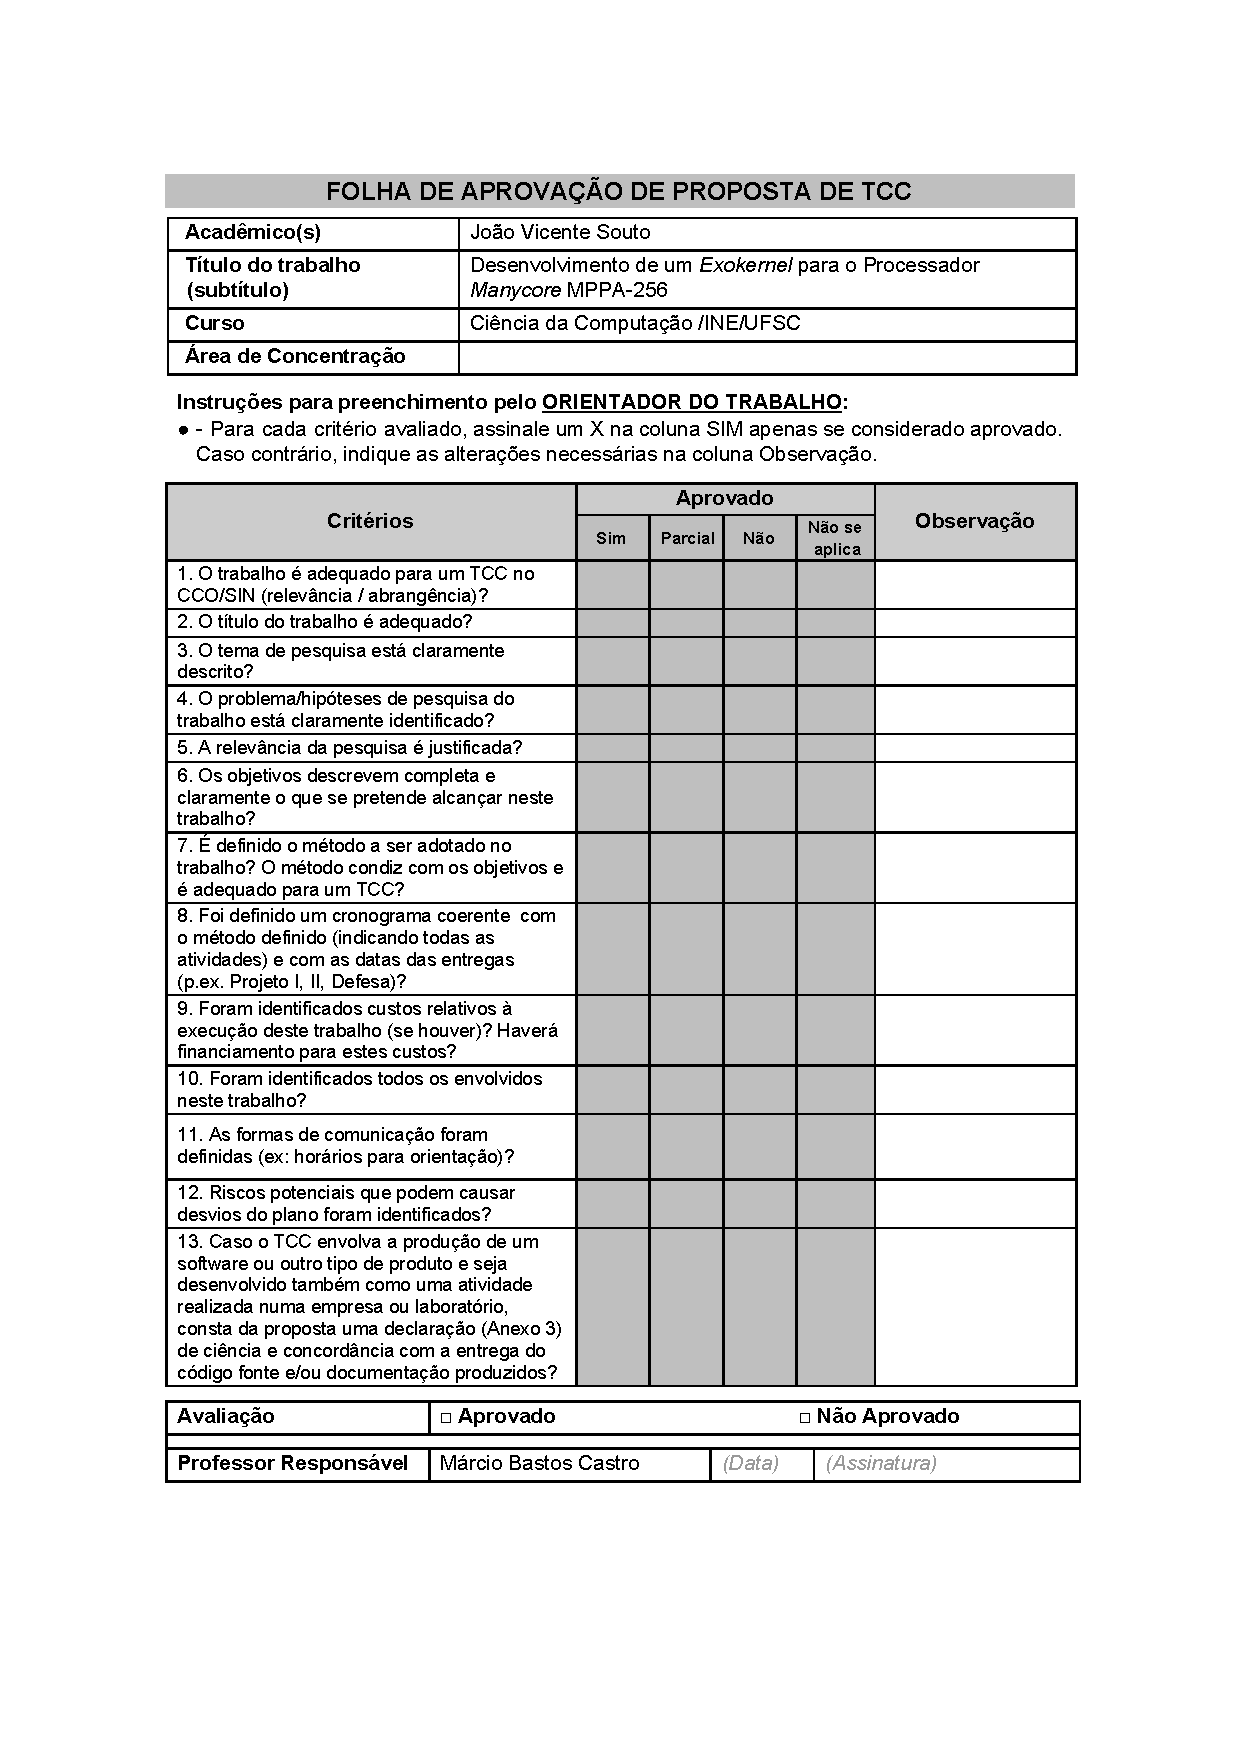
\includepdf{template_aceitacao}

   %\begin{center}
   % \vspace*{0.5cm}
   % {\large\imprimirlocal}
   % \par
   % {\large\imprimirdata}
   % \vspace*{1cm}
  %\end{center}
  
\end{folhadeaprovacao}
% ---

% ---
% Dedicatória
% ---
% \begin{dedicatoria}
%    \vspace*{\fill}
%    \centering
%    \noindent
%    \textit{ Este trabalho é dedicado às crianças adultas que,\\
%    quando pequenas, sonharam em se tornar cientistas.} \vspace*{\fill}
% \end{dedicatoria}
% ---

% ---
% Agradecimentos
% ---
% \begin{agradecimentos}
% Os agradecimentos principais são direcionados à Gerald Weber, Miguel Frasson,
% Leslie H. Watter, Bruno Parente Lima, Flávio de Vasconcellos Corrêa, Otavio Real
% Salvador, Renato Machnievscz\footnote{Os nomes dos integrantes do primeiro
% projeto abn\TeX\ foram extraídos de
% \url{http://codigolivre.org.br/projects/abntex/}} e todos aqueles que
% contribuíram para que a produção de trabalhos acadêmicos conforme
% as normas ABNT com \LaTeX\ fosse possível.

% Agradecimentos especiais são direcionados ao Centro de Pesquisa em Arquitetura
% da Informação\footnote{\url{http://www.cpai.unb.br/}} da Universidade de
% Brasília (CPAI), ao grupo de usuários
% \emph{latex-br}\footnote{\url{http://groups.google.com/group/latex-br}} e aos
% novos voluntários do grupo
% \emph{\abnTeX}\footnote{\url{http://groups.google.com/group/abntex2} e
% \url{http://abntex2.googlecode.com/}}~que contribuíram e que ainda
% contribuirão para a evolução do \abnTeX.

% Os agradecimentos

% \end{agradecimentos}
% ---

% ---
% Epígrafe
% ---
%\begin{epigrafe}
%   \vspace*{\fill}
% \begin{flushright}
%   \textit{``Não vos amoldeis às estruturas deste mundo, \\
%   mas transformai-vos pela renovação da mente, \\
%   a fim de distinguir qual é a vontade de Deus: \\
%   o que é bom, o que Lhe é agradável, o que é perfeito.\\
%   (Bíblia Sagrada, Romanos 12, 2)}
% \end{flushright}
%\end{epigrafe}
% ---

% ---
% RESUMOS
% ---

% resumo em português
\begin{resumo}

    As decisões de projeto no desenvolvimento de qualquer aplicação influenciam
    diretamente seu desempenho e consumo de energia.
    Sistemas operacionais não são diferentes, incorporando um conjunto de
    decisões de projeto que, em muitos casos, são herdadas e permanecem
    inalteradas mesmo que o \textit{hardware} e o \textit{software} tenham evoluído com o
    passar dos anos.
    Pelo fato dos sistemas operacionais formarem a base de quase todas as
    pilhas de \textit{software}, suas inadequações possuem um impacto generalizado
    nos sistemas atuais \cite{hunt_singularity:_2007}. 
    
    O objetivo deste trabalho é propor um \textit{kernel} minimalista,
    denominado \textit{exokernel}, que abstraia a alocação, manipulação e
    segurança dos recursos de comunicação do processador \textit{manycore} 
    Kalray MPPA-256.
    A motivação para o seu desenvolvimento está relacionado às abstrações
    de alto nível para comunicação entre processos denominadas \ipc e disponibilizadas
    para o processador MPPA-256, onde, apesar de facilitar o desenvolvimento
    de aplicações paralelas e distribuídas, elas dependem de uma pilha de
    \textit{software} excessiva.
    Como alternativa, é possível recorrer as bibliotecas de baixo nível que
    são utilizadas por tais abstrações, porém, características como alocação,
    sincronização, multiplexação e segurança dos recursos necessários,
    aumentam a complexidade do desenvolvimento e diminuem a portabilidade das
    aplicações.
    Neste ponto, o \textit{exokernel} fornecerá as mesmas abstrações \ipc
    disponíveis com uma comunicação entre processos eficiente, agregado a
    uma quantidade menor de camadas de \textit{software} intermediárias e conservando
    a facilidade e portabilidade existentes.
    
    Diversos experimentos serão efetuados com as abstrações disponibilizadas
    pela Kalray e implementadas pelo \textit{exokernel} proposto, com o propósito
    de comparar as duas soluções.
    A análise ocorrerá sobre métricas relevantes para o projeto, buscando
    avaliar, principalmente, o aumento do desempenho e eficiência energética
    do processador MPPA-256.

 \vspace{\onelineskip}
    
 \noindent
 \textbf{Palavras-chaves}: \textit{manycores}. MPPA-256. \textit{exokernel}. \textit{lightweight}. \textit{comunicação}. \textit{IPC}.
\end{resumo}

% resumo em inglês
% \begin{resumo}[Abstract]
%  \begin{otherlanguage*}{english}
%    This is the english abstract.

%    \vspace{\onelineskip}
 
%    \noindent 
%    \textbf{Key-words}: latex. abntex. text editoration.
%  \end{otherlanguage*}
% \end{resumo}

% ---
% inserir lista de ilustrações
% ---
%\pdfbookmark[0]{\listfigurename}{lof}
%\listoffigures*
%\cleardoublepage
% ---

% ---
% inserir lista de tabelas
% ---
%\pdfbookmark[0]{\listtablename}{lot}
%\listoftables*
%\cleardoublepage
% ---

% ---
% inserir lista de abreviaturas e siglas
% ---
%\begin{siglas}
%  \item[Fig.] Area of the $i^{th}$ component
%  \item[456] Isto é um número
%  \item[123] Isto é outro número
%  \item[lauro cesar] este é o meu nome
%\end{siglas}
% ---

% ---
% inserir lista de símbolos
% ---
%\begin{simbolos}
%  \item[$ \Gamma $] Letra grega Gama
%  \item[$ \Lambda $] Lambda
%  \item[$ \zeta $] Letra grega minúscula zeta
%  \item[$ \in $] Pertence
%\end{simbolos}
% ---

% ---
% inserir o sumario
% ---
\pdfbookmark[0]{\contentsname}{toc}
\tableofcontents*
\cleardoublepage
% ---



% ----------------------------------------------------------
% ELEMENTOS TEXTUAIS
% ----------------------------------------------------------
\textual


% ----------------------------------------------------------
% Introdução
% ----------------------------------------------------------
% \chapter{Projeto}
% \section{Introdução}
% \label{sec:introducao}

\chapter{Introdução}
\label{cap:introducao}

    Nas últimas décadas, a medida que os limites de melhoria para um único
    núcleo de processamento começaram a ser alcançados, o desenvolvimento
    de arquiteturas paralelas, possuindo processadores com centenas e até
    milhares de núcleos, supriu a crescente necessidade de poder de
    processamento das plataformas de \hpc.
    No entanto, o aumento da capacidade computacional foi acompanhada pelo
    aumento no consumo de energia, tornando-se a maior desvantagem para
    plataformas \hpc.
    
    Em uma era em que os computadores alcançaram o Petaflop, um relatório
    feito pelo Departamento de Defesa do Governo dos Estados Unidos
    (DARPA/IPTO) \cite{darpa:exascale}, mostra o aumento da preocupação
    com o consumo de energia à medida que se torna mais importante ter uma
    relação equilibrada entre poder de processamento e eficiência energética a fim de
    atingirmos o \textit{Exascale}. Em virtude disso, pesquisas científicas
    e industriais voltaram sua atenção para a aplicabilidade de arquiteturas
    \textit{manycore} de baixo consumo em problemas que demandam alto
    desempenho \cite{Castro-SBAC-PAD:2014, Castro-PARCO:2016}.
    
    Essa nova classe de arquiteturas \textit{manycore} de baixo consumo
    energético apresentam diversas características distintas das arquiteturas
    \textit{multicore} e \textit{manycore} existentes, tais como: 
    (i) centenas ou até mesmo milhares de núcleos de processamento
    simplificados em um único \textit{chip};
    (ii) comunicação entre núcleos baseada em troca de mensagens usando
    uma \noc; e 
    (iii) possuem subsistemas de memória restritiva.
    Embora a relação entre poder de processamento e eficiência energética
    seja vantajosa, tais características dificultam o desenvolvimento de aplicações
    paralelas e distribuídas para essas arquiteturas
     \cite{Castro-Souza-CCPE:2016, Castro-PARCO:2016, os:rmen}.
    
    Além dos aspectos de \textit{hardware}, aspectos de \textit{software} também influenciam
    no desenvolvimento e, principalmente, no desempenho de aplicações para
    qualquer arquitetura.
    Decisões de projeto, nível de abstração utilizado e sistema operacional
    escolhido, por exemplo, podem causar uma sobrecarga indesejada na execução
    de uma determinada aplicação \cite{Appel:1991:VMP:106972.106984, Cao:1994:IPA:1267638.1267651, Harty:1992:APM:143365.143511, Krueger:1993:TDA:165854.165867, Stonebraker:1981:OSS:358699.358703, Levy:Exception, hunt_singularity:_2007}.
    Além disso, mesmo que a aplicação utilize adequadamente todos os recursos
    disponíveis, ela deixará de explorar possíveis otimizações do seu
    domínio por não possuir acesso direto ao recursos do \textit{hardware}.
    
    Como alternativa, muitas vezes existe a opção de utilizar bibliotecas
    de baixo nível que permitem a elaboração personalizada do ambiente de
    execução, otimizando ao máximo o seu desempenho. Contudo, ao optar por se
    aproximar de uma plataforma específica, a portabilidade e complexidade do
    desenvolvimento se tornam um fator crítico ao projeto.
    
    Neste contexto, o problema de gerenciamento e proteção dos recursos de
    \textit{hardware} associado a um nível de abstração que não comprometa o desempenho
    de aplicações para processadores \textit{manycore} de baixo consumo
    energético permanece em discussão.
    Uma alternativa viável é o desenvolvimento de um \textit{exokernel} que
    concretize, através do uso de bibliotecas de baixo nível, uma camada de
    abstração de \textit{hardware} consistente e minimalista denominada \hal.

\chapter{Objetivos}
\label{cap:objetivos}

    Atualmente a Kalray disponibiliza dois ambientes de execução que
    proporcionam facilidades no desenvolvimento de aplicações paralelas
    e distribuídas para o processador MPPA-256.
    Porém, tais ambientes inferem uma sobrecarga no desempenho das aplicações
    e forçam o desenvolvedor a lidar com as decisões de projeto definidas
    pelos projetistas da Kalray.
    
    O presente trabalho tem como objetivo propor um ambiente de execução alternativo que
    equilibre flexibilidade, funcionalidade, desempenho e eficiência energética
    para o processador MPPA-256.
    Desta forma, ao utilizar camadas mais próximas do \textit{hardware} e exportar e
    proteger os recursos físicos através de uma camada de abstração,
    o \textit{exokernel} proposto proporcionará maior liberdade ao
    desenvolver em explorar otimizações para o domínio de aplicações de \hpc e,
    ao mesmo tempo, não aumentará a complexidade do projeto por
    não trabalhar diretamente com um \textit{hardware} específico.
    
    O \textit{exokernel} deverá, dada a utilização das primitivas \ipc para
    comunicação e sincronização entre processos em \textit{clusters} distintos,
    realizar a alocação, proteção e multiplexação dos recursos necessários, 
    além da configuração e envio/recebimento de dados.
    Ao prover a comunicação, o \textit{exokernel} deverá implementar uma 
    política de troca de mensagens assíncronas abaixo de sua interface, 
    a fim de providenciar uma comunicação eficiente e não provocar perda de
    desempenho ou eficiência energética em relação aos ambientes de execução
    existentes.
    Para isso, serão utilizadas bibliotecas de baixo nível do processador MPPA-256.
    
    \begin{flushleft}
    \textbf{Restrições:}
    \begin{itemize}
        \item Executar aplicações no processador;
        \item Utilizar as bibliotecas de baixo nível do processador;
        \item Memória limitada no \textit{chip}, dividida entre o sistema operacional e a aplicação;
        \item Respeitar as datas de entregas.
    \end{itemize}
    
    \textbf{Premissas:}
    \begin{itemize}
        \item Processador disponível;
        \item Documentação disponível;
        \item Acesso ao processador de forma remota; 
        \item Computador disponível; 
        \item Disponibilidade de água, luz e energia;
        \item Acesso à Internet.
    \end{itemize}
    
    \textbf{Marcos:}
    \begin{itemize}
        \item Entrega da proposta: 12-11-2018;
        \item Entrega do resumo em TCC I: junho de 19; 
        \item Primeira entrega da monografia em TCCII: outubro de 19; 
        \item Apresentação da monografia: novembro de 19;
        \item Segunda entrega da monografia em TCCII (versão final): dezembro de 19.
    \end{itemize}
    
    \textbf{Critérios de aceite:}
    \begin{itemize}
        \item Aprovação pela banca;
        \item Aprovação do orientador;
        \item Conformidade com as normas definidas pela instituição;
        \item Prazos cumpridos;
        \item Entregas cumpridas.
    \end{itemize}
    \end{flushleft}


\chapter{Fundamentação Teórica}
\label{sec:fundamentacao}

    Esta seção apresenta uma fundamentação teórica básica sobre o
    principal objeto de estudo (Seção \ref{sec:mppa}) e conceito necessário
    (Seção \ref{sec:exokernel}) para a viabilidade deste projeto.

    \section{Processador \textit{manycore} MPPA-256}
    \label{sec:mppa}
    
        % FIGURA DA ARQUITETURA
        \begin{figure}[t]
            \begin{center}
                \caption{Visão geral do MPPA-256.}
                    \label{figmppa}
                \begin{tabular}{ccc}
                    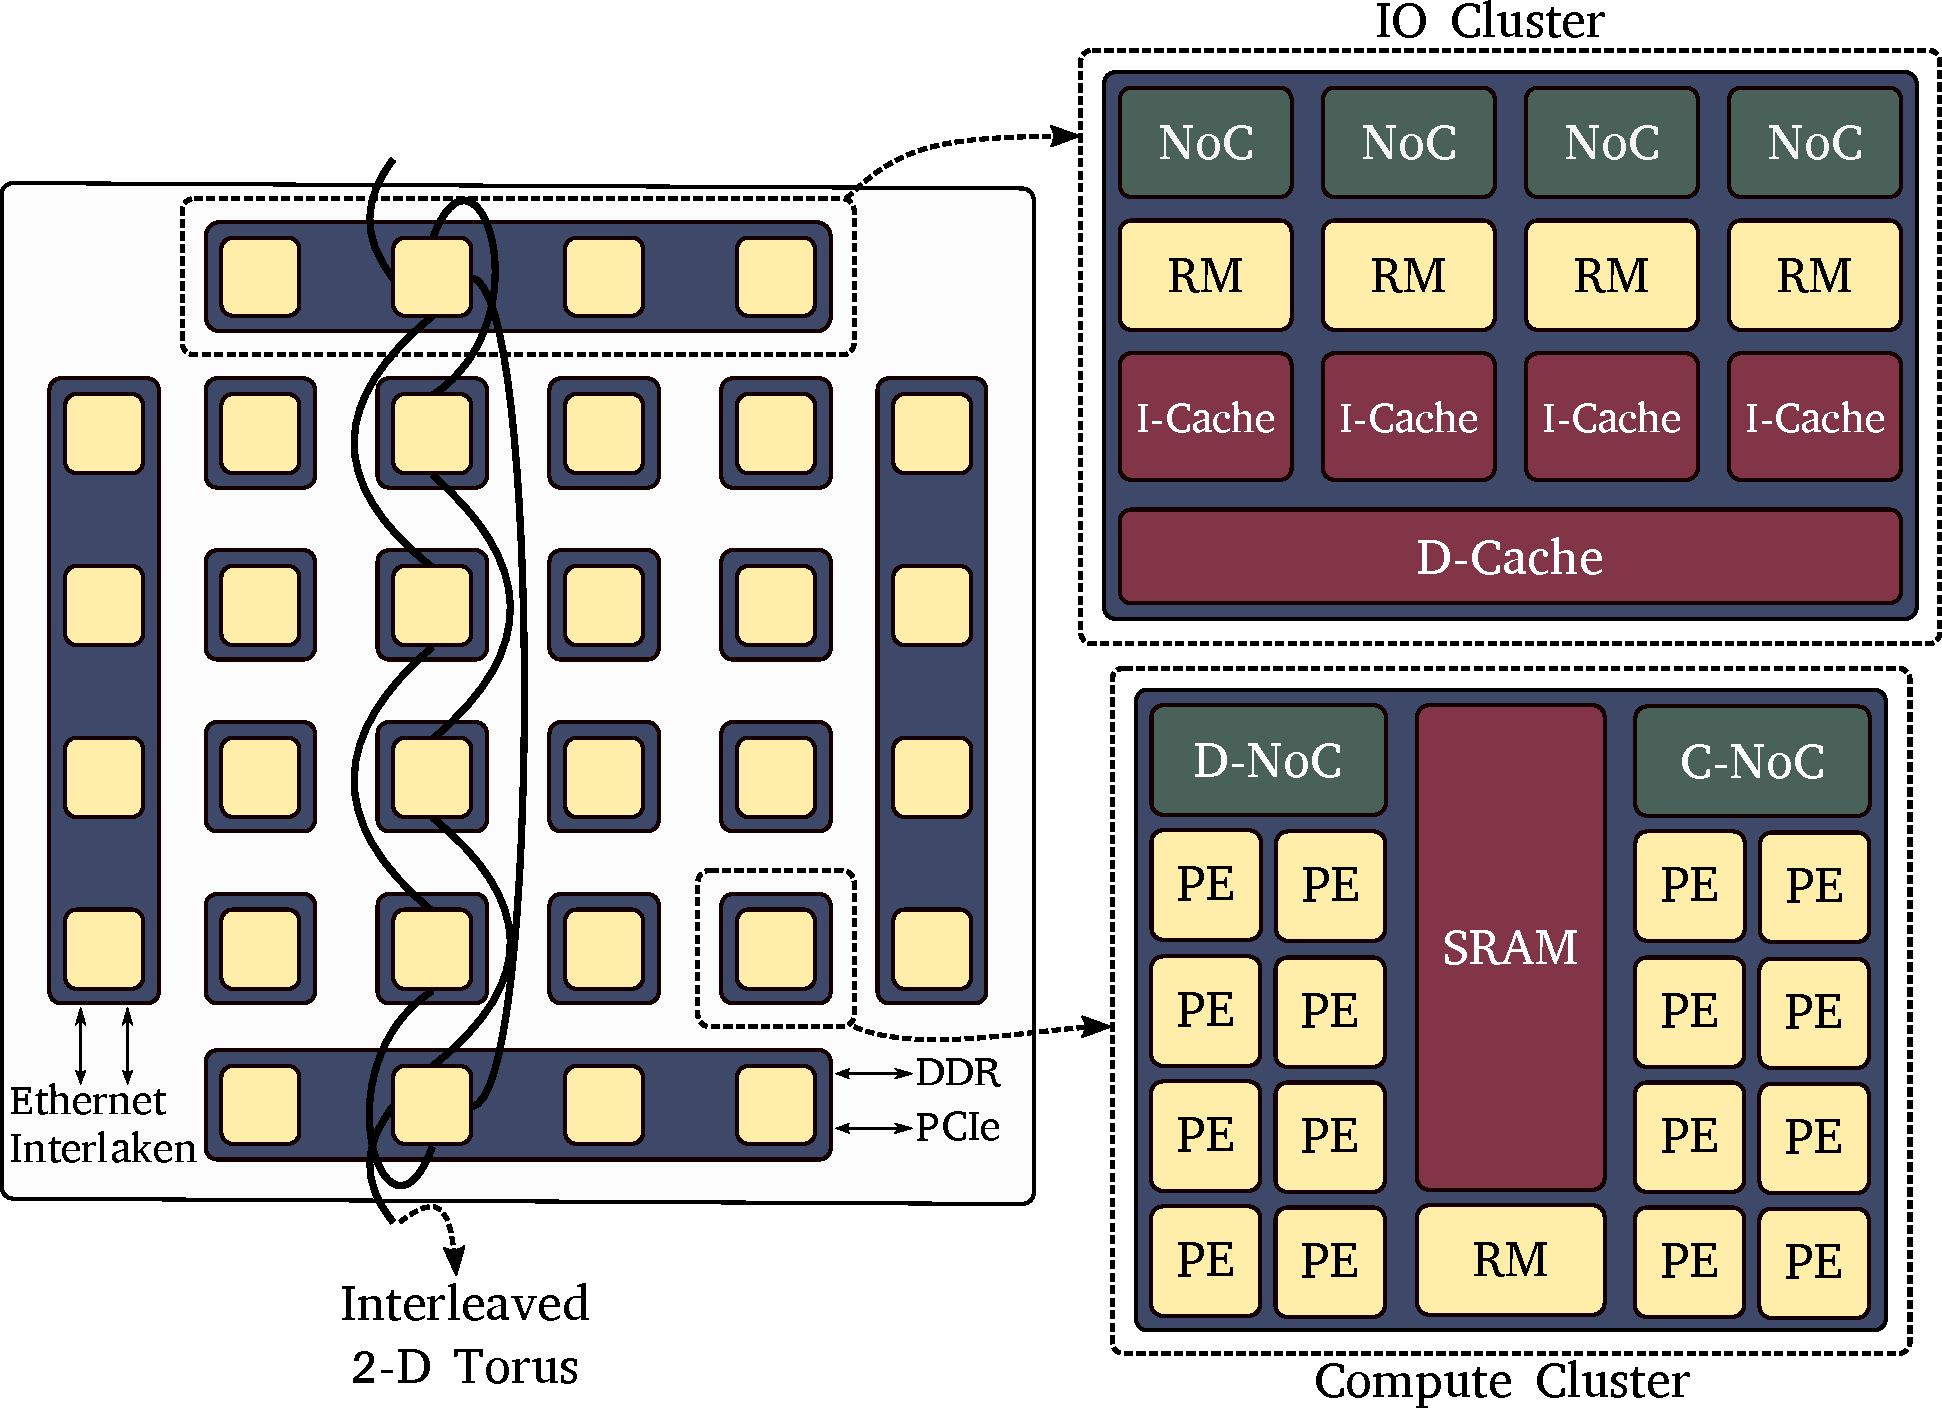
\includegraphics[width=0.5\textwidth]{figs/mppa-overview.pdf}\\
                \end{tabular}
                \vspace{1ex} \\
                Fonte: (\citeonline{os:rmen})
            \end{center}
            \vspace{-2ex}
        \end{figure}
    
        O processador MPPA-256 é um exemplo de arquitetura \textit{manycore}
        de baixo consumo energético \cite{Castro-IA3:2013} desenvolvido pela
        empresa francesa Kalray. Como mostra a Figura \ref{figmppa}, o MPPA-256
        é um processador que integra 256 núcleos de propósito geral,
        denominados \pes, e 32 núcleos dedicados ao sistema operacional,
        denominados \rmans, criados sobre uma tecnologia CMOS de 28nm.
        Esses núcleos são distribuídos através de 16 \textit{clusters} de
        computação (\cpclusters) com 16 \pes e 1 \rman cada, somados a 
        4 \textit{quad-cores} para os subsistemas de E/S (\ioclusters).
        Cada \textit{cluster} possui um espaço de endereçamento privado,
        enquanto as comunicações ocorrem através de uma \noc dedicada a
        dados, denominada \dnoc, e outra dedicada a controles, denominada \cnoc.
            
        As camadas de \textit{software} disponibilizadas para o processador MPPA-256,
        como pode ser visto na Figura \ref{figruntime}, possuem
        (i) suporte a programação paralela e distribuída, como
        \textit{POSIX}, \textit{OpenMP} etc;
        (ii) primitivas para sincronização e comunicação entre processos
        (\ipc), tais como, \textit{sync}, \textit{portal} e \textit{mailbox};
        (iii) sistemas operacionais para cada tipo de \textit{cluster}; e
        (iv) acesso aos recursos do \textit{hardware} através de bibliotecas de baixo nível.

        % FOTO DA SOFTWARE STACK
        \begin{figure}[b]
          \begin{center}
              \caption{Ambiente de execução do processador MPPA-256.}
                   \label{figruntime}
            \begin{tabular}{ccc}
              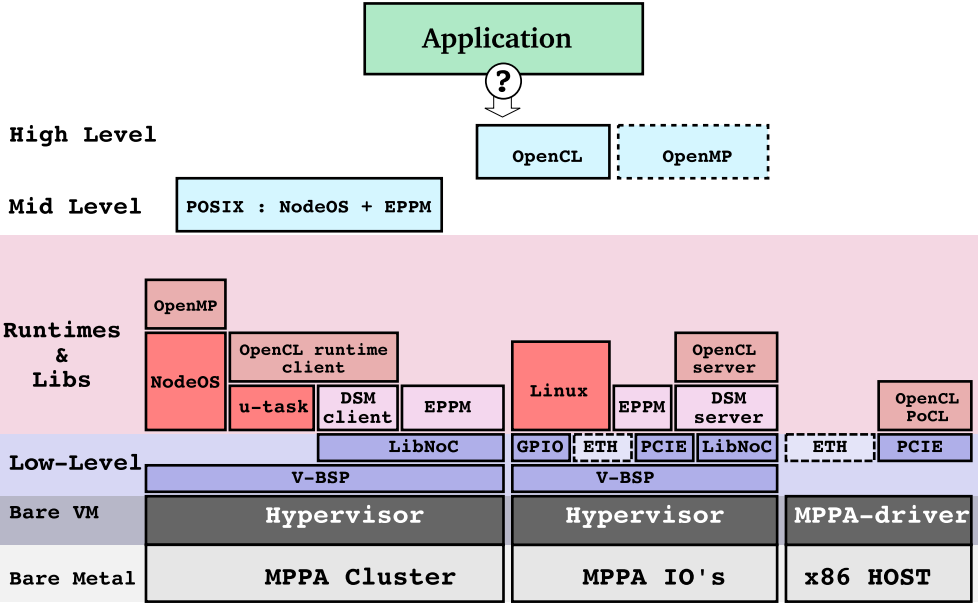
\includegraphics[width=0.6\textwidth]{figs/software_stack.png} \\
            \end{tabular}
                \vspace{1ex} \\
                Fonte: Documentação do processador MPPA-256
            \end{center}
           \vspace{-2ex}
        \end{figure}

        Nos \ioclusters, é possível executar uma variação do sistema
        operacional Linux, nomeada \rtems, possibilitando a comunicação da
        máquina \textit{host} com o dispositivo, além da comunicação
        com os \cpclusters.
        Sobre outra perspectiva, nos \cpclusters, o sistema operacional
        \nodeos, projetado para adequar-se aos 2-MB de memória local, é executado 
        no \rman com o objetivo de auxiliar e gerenciar a comunicação dos \pes
        com os demais elementos do processador.
        Em alternativa a esses ambientes de execução, existe a possibilidade
        de utilizar o processador MPPA-256 apenas com o \textit{hypervisor} 
        e o auxílio de bibliotecas de baixo nível.
        
        A comunicação entre processos em \textit{clusters} distintos ocorre
        de maneira explícita, principalmente  através de três primitivas \ipc.
        Entre elas estão,
        (i) \textit{Sync}: permite a sincronização de \textit{N:M} processos através da \cnoc;
        (ii) \textit{Mailbox}: envio de mensagens pequenas através da \dnoc; e
        (iii) \textit{Portal}: envio de grandes quantidade de dados através da \dnoc.
        De forma semelhante aos sistemas operacionais, o desenvolvedor tem a
        liberdade de lidar com bibliotecas de baixo nível que são utilizadas
        por essas primitivas.
    
    \section{Exokernel}
    \label{sec:exokernel}
    
        O \textit{Exokernel} consiste em uma arquitetura desenvolvida
        pelo \unimit que exporta com segurança todos os
        recursos de \textit{hardware} através de uma interface de baixo nível.
        Seu objetivo é proporcionar o gerenciamento de recursos físicos
        no nível da aplicação em oposição a limitação do desempenho, da
        flexibilidade e da funcionalidade impostas por sistemas operacionais 
        tradicionais.

        Ao contrário da abordagem comum escolhida por sistemas operacionais
        monolíticos, expondo os recursos de \textit{hardware} através de abstrações
        de alto nível, o \textit{Exokernel} transfere a responsabilidade de
        implementá-las para o desenvolver da aplicação, como pode ser visto
        na Figura \ref{figexokernel}.
        Neste ponto, o \textit{Exokernel} também se opõe a ideia dos 
        \textit{microkernels}, que, ao contrário de buscar fornecer as
        mesmas abstrações de sistemas monolíticos com uma quantidade menor
        de camadas intermediárias, propõe apenas separar a função de proteção
        dos recursos do \textit{hardware} da função de gerenciamento.
        Desta forma, ao não impor abstrações ao desenvolvedor, permite a
        personalização do ambiente de execução em prol do domínio da aplicação.
                
        Por fim, a arquitetura de \textit{software} definida pelo \textit{Exokernel}
        provou ser uma alternativa viável às arquiteturas de sistemas
        operacionais tradicionais demonstrando que, 
        (i) um número limitado de primitivas simplificadas permite 
        implementa-las eficientemente; 
        (ii) a proteção dos recursos pode ser realizada de forma eficaz com
        implementações de baixo nível; (iii) abstrações tradicionais de
        sistemas operacionais podem ser desenvolvidas em cima dessas
        primitivas de forma eficiente; e 
        (iv) permite que aplicações desenvolvam abstrações de propósito
        geral através de pequenas modificações \cite{engler_exokernel:_1995}.

        % FOTO DO EXOKERNEL
        \begin{figure}[t]
          \begin{center}
              \caption{Arquitetura \textit{Exokernel}.}
                   \label{figexokernel}
            \begin{tabular}{ccc}
                  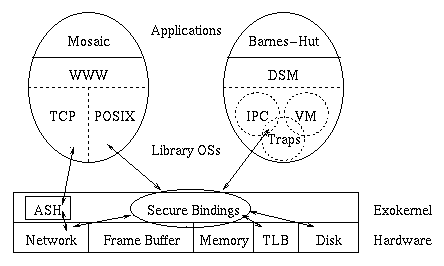
\includegraphics[width=0.4\textwidth]{figs/exokernel.png} \\
            \end{tabular}
                \vspace{1ex} \\
                Fonte: \cite{misc:exokernel}
            \end{center}
           \vspace{-2ex}
        \end{figure}

\chapter{Método de Pesquisa}
\label{cap:metodo-pesquisa}

    O andamento deste projeto ocorrerá em paralelo à pesquisa de doutorado do
    coorientador deste projeto, Pedro Henrique Penna, e utilizará como base o
    protótipo do sistema operacional distribuído, denomidado \textit{multikernel},
    implementando no repositório do sistema operacional Nanvix \cite{Penna2017,Penna2017-1}
    disponibilizado em \url{https://github.com/nanvix/multikernel}.
    
    O desenvolvimento do trabalho será feito na linguagem C e dividido em
    cinco módulos, os quais são,
    (i) \textit{\noc Driver}: utilização da biblioteca de baixo nível da \noc
    para controle, manipulação e multiplexação dos \textit{buffers} de comunicação;
    (ii) \textit{Core Driver}: identificação e configuração dos elementos ativos 
    do sistemas (\ioclusters e \cpclusters); 
    (iii) \textit{Sync}: abstração para sincronização entre processos localizados
    em \textit{clusters} distintos;
    (iv) \textit{Mailbox}: abstração para troca de mensagens pequenas, geralmente 
    associadas a operações de controle; e 
    (v) \textit{Portal}: abstração dedicada a troca de dados intensa. 
    Os módulos \textit{sync} e \textit{mailbox} são dependentes dos dois
    primeiros módulos, assim como o \textit{portal} é dependente dos demais.
    
    Os módulos e testes desenvolvidos utilizarão as bibliotecas e documentação
    disponibilizados pela Kalray e serão executados no processador MPPA-256.
    A plataforma que contém o MPPA-256 está localizada em Grenoble (França) e o acesso
    remoto é proporcionado por uma parceria entre o \lapesd e o \lig.
    O orientando terá acesso ao laboratório \lapesd, localizado na Universidade
    Federal de Santa Catarina (UFSC), no qual possuirá uma máquina disponível
    para o desenvolvimento do trabalho.
    Além disso, o andamento deste trabalho ocorrerá associado a bolsa
    de iniciação científica do orientando, contribuindo com a sua formação e
    na qualidade final do trabalho desenvolvido.

% ----------------------------------------------------------
% PARTE - preparação da pesquisa
% ----------------------------------------------------------
% \part{Preparação da pesquisa}

% ----------------------------------------------------------
% Capitulo com exemplos de comandos inseridos de arquivo externo 
% ----------------------------------------------------------

\include{abntex2-modelo-include-comandos}

% ----------------------------------------------------------
% Parte de revisãod e literatura
% ----------------------------------------------------------
% \part{Revisão de Literatura}

% ---
% Capitulo de revisão de literatura
% ---
\chapter{Planejamento}

Este capítulo apresenta planejamento do trabalho, o qual é composto pelo cronograma de atividades, os recursos humanos necessários e os seus custos. Além disso, serão descritas as atividades de comunicação necessárias para a execução do projeto, assim como os possíveis riscos associados às atividades.

% ---
\section{Cronograma}

\newcommand{\cc}{\cellcolor{black!25}}  % Color cell
\arrayrulecolor{black}                  % Color lines


\begin{table}[b]
\resizebox{\textwidth}{!}{
    \begin{tabular}{|l|c|c|c|c|c|c|c|c|c|c|c|c|c|c|c|}
    \hline
           & \multicolumn{3}{c|}{2018} & \multicolumn{12}{c|}{2019}\\ \hline
           
    Etapas/Meses            & 10  & 11  & 12  & 01  & 02  & 03  & 04  & 05  & 06  & 07  & 08  & 09  & 10  & 11  & 12  \\ \hline
    Desenvolv. da Solução   & \cc & \cc & \cc & \cc & \cc & \cc & \cc & \cc & \cc & \cc &     &     &     &     &     \\ \hline
    Relatório Projeto I     &     &     &     &     &     &     &     & \cc & \cc &     &     &     &     &     &     \\ \hline
    Conclusões              &     &     &     &     &     &     &     &     &     & \cc & \cc &     &     &     &     \\ \hline
    Rascunho Projeto II     &     &     &     &     &     &     &     &     &     &     &     & \cc & \cc &     &     \\ \hline
    Defesa                  &     &     &     &     &     &     &     &     &     &     &     &     &     & \cc &     \\ \hline
    Ajustes e Envio Final   &     &     &     &     &     &     &     &     &     &     &     &     &     & \cc & \cc \\ \hline
    \end{tabular}
}
\caption{Cronograma de atividades do projeto.}
\end{table}


O planejamento deste trabalho está organizado da seguinte maneira.
O desenvolvimento da solução abrange a especificação do trabalho apresentado
no Capítulo \ref{cap:metodo-pesquisa}.
O primeiro resumo da monografia, relacionado ao relatório do Projeto I, 
desenvolverá a estrutura básica da monografia e conterá os resultados obtidos
até o momento. 
As conclusões encerrarão o desenvolvimento da solução, levando em consideração
o retorno obtido do relatório do Projeto I e iniciarão a síntese dos resultados. 
O rascunho relacionado ao Projeto II envolverá as atividades de elaboração da 
monografia e o preparo da apresentação para a defesa. 
A defesa apresentará o trabalho desenvolvido e os resultados alcançados.
Por fim, serão realizados os ajustes e correções solicitados pelos membros da 
banca e a versão final da monografia será enviada ao acervo da UFSC.

% ---

% ---
\section{Recursos Humanos}

\begin{center}
\begin{tabular}{|c|c|}
\hline
    Papel              & Nome                 \\ \hline
    Orientador         & Márcio Bastos Castro \\ \hline
    Coorientador       & Pedro Henrique Penna \\ \hline
    Coordenador        & Renato Cislaghi      \\ \hline
    Membro da Banca I  & A definir            \\ \hline
    Membro da Banca II & A definir            \\ \hline
    Autor              & João Vicente Souto   \\ \hline
\end{tabular}
\end{center}
% ---

% ---
\section{Custos}

\begin{center}
\begin{tabular}{|c|c|c|c|c|c|}
\hline
\multicolumn{6}{|c|}{Estimativas para Recursos Humanos} \\ \hline
    Nome         & Data Início & Data Fim   & Hora/Mês & Valor/Hora & Custo Total \\ \hline
    Autor        & 30/09/2018  & 15/12/2019 & 96       & R\$ 5,00   & R\$ 7200,00 \\ \hline
    Orientador   & 30/09/2018  & 15/12/2019 & 8        & R\$ 65,00  & R\$ 7800,00 \\ \hline
    Coorientador & 30/09/2018  & 15/12/2019 & 8        & R\$ 65,00  & R\$ 7800,00 \\ \hline
    Coordenador  & 30/06/2019  & 15/12/2019 & 1        & R\$ 137,00 & R\$ 959,00  \\ \hline
    Banca I      & 30/06/2019  & 15/12/2019 & 1        & R\$ 135,00 & R\$ 945,00  \\ \hline
    Banca II     & 30/06/2019  & 15/12/2019 & 1        & R\$ 135,00 & R\$ 945,00  \\ \hline
\multicolumn{5}{|l|}{Subtotal estimativas para recursos humanos} & R\$ 25.649,00 \\
\hline
\end{tabular}
\end{center}

\begin{center}
\begin{tabular}{|c|c|c|c|c|c|}
\hline
\multicolumn{6}{|c|}{Estimativas para Recursos Não Humanos} \\ \hline
    Descrição & Data Início & Data Fim & Quantidade & Valor Unitário & Custo Total \\
    \hline
    CDs       & 12/19 & 12/19 & 2 & R\$ 3,00  & R\$ 6,00 \\ \hline
    Impressão & 12/19 & 12/19 & 3 & R\$ 15,00 & R\$ 45,00 \\ \hline
\multicolumn{5}{|l|}{Subtotal estimativas para recursos não humanos} & R\$ 51,00 \\
\hline
\end{tabular}
\end{center}
% ---

% ---
\section{Comunicação}

\begin{center}
\begin{tabular}{|l|p{9cm}|}
\hline
    O que precisa ser comunicado & Entrega da Proposta \\ \hline
    Emissor & João Vicente Souto \\ \hline
    Receptor & Renato Cislaghi \\ \hline
    Comunicação & Será entregue a proposta completa do TCC \\ \hline
    Forma de comunicação & Sistema de TCC \\ \hline
    Frequência ou Quando & Única vez \\ \hline
\end{tabular}
\end{center}

\begin{center}
\begin{tabular}{|l|p{9cm}|}
\hline
    O que precisa ser comunicado & Entrega do Relatório em TCC I \\ \hline
    Emissor & João Vicente Souto \\ \hline
    Receptor & Renato Cislaghi \\ \hline
    Comunicação & Será entregue a primeira parte da monografia \\ \hline
    Forma de comunicação & Sistema de TCC \\ \hline
    Frequência ou Quando & Única vez \\ \hline
\end{tabular}
\end{center}

\begin{center}
\begin{tabular}{|l|p{9cm}|}
\hline
    O que precisa ser comunicado & Entrega da mografia completa em TCC II \\ \hline
    Emissor & João Vicente Souto \\ \hline
    Receptor & Renato Cislaghi \\ \hline
    Comunicação & Será entregue a monografia completa \\ \hline
    Forma de comunicação & Sistema de TCC \\ \hline
    Frequência ou Quando & Única vez \\ \hline
\end{tabular}
\end{center}

\begin{center}
\begin{tabular}{|l|p{9cm}|}
\hline
    O que precisa ser comunicado & Defesa do TCC \\ \hline
    Emissor & João Vicente Souto \\ \hline
    Receptor & Márcio Bastos Castro, Membro da Banca I, Membro da Banca II\\ \hline
    Comunicação & Será feita a defesa do TCC aos membros da banca.  \\ \hline
    Forma de comunicação & Pessoalmente \\ \hline
    Frequência ou Quando & Única vez \\ \hline
\end{tabular}
\end{center}

\begin{center}
\begin{tabular}{|l|p{9cm}|}
\hline
    O que precisa ser comunicado & Reuniões com o Orientador \\ \hline
    Emissor & João Vicente Souto \\ \hline
    Receptor & Márcio Bastos Castro \\ \hline
    Comunicação & Reuniões com o orientador para atualizações e dúvidas \\ \hline
    Forma de comunicação & Pessoalmente \\ \hline
    Frequência ou Quando & Quinzenalmente \\ \hline
\end{tabular}
\end{center}

\begin{center}
\begin{tabular}{|l|p{9cm}|}
\hline
    O que precisa ser comunicado & Reuniões com o Coorientador \\ \hline
    Emissor & João Vicente Souto \\ \hline
    Receptor & Pedro Henrique Penna \\ \hline
    Comunicação & Reuniões com o coorientador para atualizações e dúvidas \\ \hline
    Forma de comunicação & Videoconferência \\ \hline
    Frequência ou Quando & Semanalmente \\ \hline
\end{tabular}
\end{center}

\begin{center}
\begin{tabular}{|l|p{9cm}|}
\hline
    O que precisa ser comunicado & Enviar a monografia com ajustes após a defesa \\ \hline
    Emissor & João Vicente Souto \\ \hline
    Receptor & Renato Cislaghi \\ \hline
    Comunicação & Entrega da monografia com os ajustes necessários \\ \hline
    Forma de comunicação & Sistema de TCC \\ \hline
    Frequência ou Quando & Única vez \\ \hline
\end{tabular}
\end{center}
% ---

% ---
\newpage
\section{Riscos}

\begin{center}
\resizebox{\textwidth}{!}{
\begin{tabular}{|l|c|c|c|c|l|}
\hline
    Nome & Probabilidade & Impacto & Exposição & 
    Estratégia & Ações de Prevenção  \\ \hline
    
     \makecell[l]{Sobrecarga da \\ graduação} & Média & Alto & Alto & Mitigar & \makecell[l]{Cumprir o \\ cronograma \\ proposto.}\\ \hline
     \makecell[l]{O acesso à máquina\\ está offline} & Média & Médio & Médio & Mitigar & - \\ \hline
     \makecell[l]{Outra pessoa está \\ utilizando a máquina \\ por um período longo} & Média & Médio & Média & Aceitar & -\\ \hline
     \makecell[l]{Orientador está\\ de viagem} & Média & Baixo & Médio & Mitigar & - \\ \hline
     \makecell[l]{Orientador fica doente} & Média & Baixo & Baixa & Mitigar & - \\ \hline
     \makecell[l]{Greve de ônibus} & Média & Baixo & Baixa & Mitigar & \makecell[l]{Manter a \\ manutenção \\ do carro em dia.} \\ \hline
     \makecell[l]{O aluno ficou doente} & Média & Médio & Média & Aceitar & \makecell[l]{Fazer exercícios, \\ comer bem e \\ ir ao médico \\ ocasionalmente.}\\ \hline
     \makecell[l]{Computador não \\está mais funcionando} & Baixa & Médio & Média & Mitigar &\makecell[l]{ Tomar cuidado \\ ao manusear \\o computador e \\ desliga-lo \\ adequadamente.}  \\ \hline
\end{tabular}
}
\end{center}
% ---


% ----------------------------------------------------------
% Resultados
% ----------------------------------------------------------
%\part{Resultados}

% ---
% primeiro capitulo de Resultados
% ---
%\chapter{Cap 2}

% ---
%\section{S}
% ---


% ---
% segundo capitulo de Resultados
% ---
%\chapter{Cap 3}

% ---
%\section{S}
% ---


% ---
% Finaliza a parte no bookmark do PDF, para que se inicie o bookmark na raiz
% ---
\bookmarksetup{startatroot}% 
% ---

% ---
% Conclusão
% ---
%\chapter*[Conclusão]{Conclusão}
%\addcontentsline{toc}{chapter}{Conclusão}

%\lipsum[31-33]

% ----------------------------------------------------------
% ELEMENTOS PÓS-TEXTUAIS
% ----------------------------------------------------------
\postextual

% ----------------------------------------------------------
% Referências bibliográficas
% ----------------------------------------------------------
\bibliography{bibliography}

% ----------------------------------------------------------
% Glossário
% ----------------------------------------------------------
%
% Consulte o manual da classe abntex2 para orientações sobre o glossário.
%
%\glossary

% ----------------------------------------------------------
% Apêndices
% ----------------------------------------------------------

% ---
% Inicia os apêndices
% ---
%\begin{apendicesenv}

% Imprime uma página indicando o início dos apêndices
%\partapendices

% ----------------------------------------------------------
%\chapter{Quisque libero justo}
% ----------------------------------------------------------

%\lipsum[50]

% ----------------------------------------------------------
%\chapter{Nullam elementum urna vel imperdiet sodales elit ipsum pharetra ligula
%ac pretium ante justo a nulla curabitur tristique arcu eu metus}
% ----------------------------------------------------------
%\lipsum[55-57]

%\end{apendicesenv}
% ---


% ----------------------------------------------------------
% Anexos
% ----------------------------------------------------------

% ---
% Inicia os anexos
% ---
%\begin{anexosenv}

% Imprime uma página indicando o início dos anexos
%\partanexos

% ---
%\chapter{Morbi ultrices rutrum lorem.}
% ---
%\lipsum[30]

% ---
%\chapter{Cras non urna sed feugiat cum sociis natoque penatibus et magnis dis
%parturient montes nascetur ridiculus mus}
% ---

%\lipsum[31]

% ---
%\chapter{Fusce facilisis lacinia dui}
% ---

%\lipsum[32]

%\end{anexosenv}

%---------------------------------------------------------------------
% INDICE REMISSIVO
%---------------------------------------------------------------------

%\printindex

\end{document}
